\documentclass[12pt,a4paper]{article}
\usepackage[utf8]{inputenc}
\usepackage{listings}
\usepackage{graphicx}
\usepackage{authblk}
\usepackage{fancyhdr}
\usepackage{minted}
\usepackage{xcolor}

\usepackage[]{geometry}
\graphicspath{ {./images/} }
\title{IT Workshop Assignment }

\author{LEGALA SHARADHA}
\affil{B192157}
\affil{CSE-C3}

\date{August 2022}


\begin{document}

\maketitle\vskip-15pt\hrule\vskip15pt


\section{About Iris Data}
The following data includes three species iris flower with 50 samples each as well as
some properties about each flower.
The columns in this dataset are:
\begin{itemize}
\color{brown}
\item Sepal Length
\color{red}
\item Sepal Width
\color{cyan}
\item Petal width
\color{lime}
\item Petal Width
\color{teal}
\item Species
\end{itemize}

\textbf{ANALYSIS OF THE ABOVE IRIS DATA USING FEW PYTHON LIBRARIES}



\begin{minted}{python}
import matplotlib.pyplot as plt
import pandas as pd
import numpy as np
df =pd.read_csv("iris.csv")
s=len([i for i in df["variety"] if i=="Setosa"])
ve=len([j for j in df["variety"] if j=="Versicolor"])
vi=len([k for k in df["variety"] if k=="Virginica"])
plt.figure(figsize=(8,10))
plt.pie([s,ve,vi],labels=["setosa","Versicolor","Verginica"],autopct="%2.1f%%",explode=(0.1,0.1,0.1),shadow=True)
plt.title("iris Species %")
plt.ylabel("Species",labelpad=45)
plt.legend(title="varieties",loc=(1,0),shadow=True)

plt.savefig("C:\\Users\\shaik\\OneDrive\\Desktop\\itass\\pie.jpeg",bbox_inches="tight",pad_inches=0.5)
plt.show()
\end{minted}

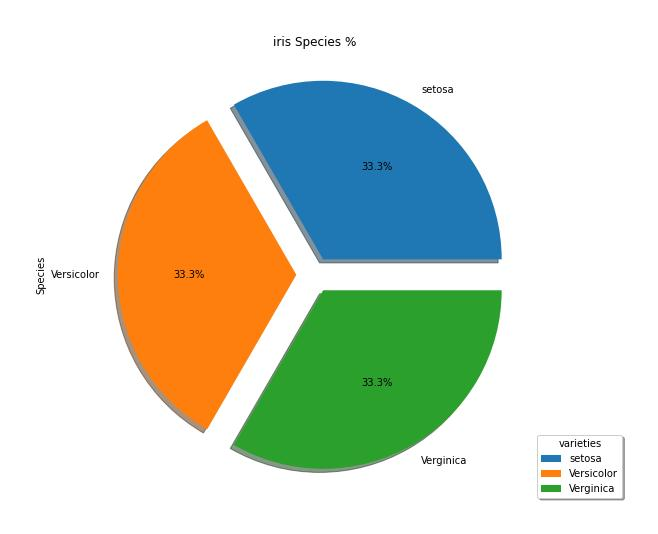
\includegraphics[width=10cm, height=8cm]{pie.jpeg}
\begin{minted}{python}
bool1=df["variety"]=="Setosa"
setosa_sl=df[bool1]["sepal.length"]
setosa_sw=df[bool1]["sepal.width"]
bool2=df["variety"]=="Versicolor"
versicolor_sl=df[bool2]["sepal.length"]
versicolor_sw=df[bool2]["sepal.width"]
bool3=df["variety"]=="Virginica"
virginica_sl=df[bool3]["sepal.length"]
virginica_sw=df[bool3]["sepal.width"]
plt.figure(figsize=(10,10))
plt.scatter(setosa_sl,setosa_sw,c="r",label="iris setosa")
plt.scatter(versicolor_sl,versicolor_sw,c="g",label="iris versicolor")
plt.scatter(virginica_sl,virginica_sw,c="b",label="iris virginica")
plt.legend(shadow=True,frameon=True,loc=1)
plt.grid(linestyle=":")

plt.title(" The iris Data set")
plt.xlabel("sepal length")
plt.ylabel("sepal width")
plt.xlim(4.0)
plt.ylim(1.5)
plt.savefig("C:\\Users\\shaik\\OneDrive\Desktop\\itass\\scatter.jpeg",bbox_inches="tight",pad_inches=0.5)
plt.show()
\end{minted}
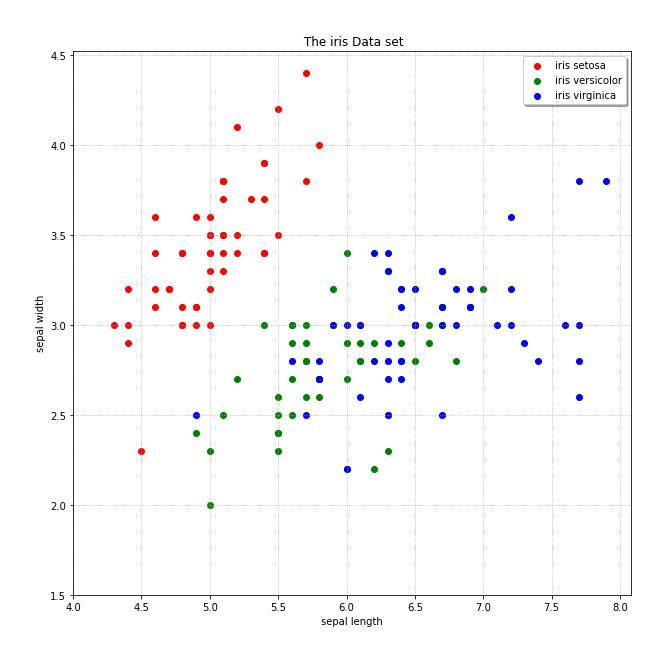
\includegraphics[width=15cm,height=15cm]{scatter.jpeg}
\begin{minted}{python}
bool1=df["variety"]=="Setosa"
setosa_sl=df[bool1]["sepal.length"]
setosa_sw=df[bool1]["sepal.width"]
bool2=df["variety"]=="Versicolor"
versicolor_sl=df[bool2]["sepal.length"]
versicolor_sw=df[bool2]["sepal.width"]
bool3=df["variety"]=="Virginica"
virginica_sl=df[bool3]["sepal.length"]
virginica_sw=df[bool3]["sepal.width"]
plt.figure(figsize=(10,10))
plt.scatter(setosa_sl,setosa_sw,c="r",label="iris setosa")
plt.scatter(versicolor_sl,versicolor_sw,c="g",label="iris versicolor")
plt.scatter(virginica_sl,virginica_sw,c="b",label="iris virginica")
plt.legend(shadow=True,frameon=True,loc=1)
plt.grid(linestyle=":")

plt.title(" The iris Data set")
plt.xlabel("sepal length")
plt.ylabel("sepal width")
plt.xlim(4.0)
plt.ylim(1.5)
plt.savefig("C:\\Users\\shaik\\OneDrive\Desktop\\itass\\scatter.jpeg",bbox_inches="tight",pad_inches=0.5)
plt.show()
\end{lstlisting}
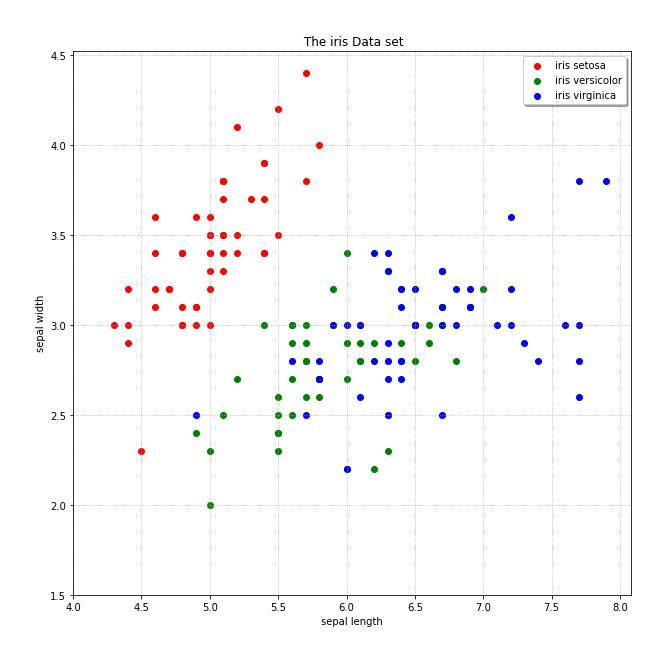
\includegraphics[width=15cm,height=15cm]{scatter.jpeg}
\begin{lstlisting}[language=Python]
bool4=df["variety"]=="Setosa"

setosa_pl=df[bool4]["petal.length"]
setosa_pw=df[bool4]["petal.length"]
bool5=df["variety"]=="Versicolor"
versicolor_pl=df[bool5]["petal.length"]
versicolor_pw=df[bool5]["petal.length"]
bool6=df["variety"]=="Virginica"
virginica_pl=df[bool6]["petal.length"]

virginica_pw=df[bool6]["petal.width"]
def avg(li):
    return sum(li)/len(li)
plt.figure(figsize=(10,10))
x=["sepal length","sepal width","petal length","petal width"]
h1=[avg(setosa_sl),avg(setosa_sw),avg(setosa_pl),avg(setosa_pw)]
h2=[avg(versicolor_sl),avg(versicolor_sw),avg(versicolor_pl),avg(versicolor_pw)]
h3=[avg(virginica_sl),avg(virginica_sw),avg(virginica_pl),avg(virginica_pw)]
w=0.2
bar1=np.arange(len(x))
bar2=[i+w for i in bar1]
bar3=[j+w for j in bar2]
plt.bar(bar1,h,w,label="setosa")
plt.bar(bar2,h2,w,label="versicolor")
plt.bar(bar3,h3,w,label="verginica")
plt.xticks(bar1+w,x)
plt.xlabel('Features',size=15)
plt.ylabel("value in cm.",size=15)
plt.title("average heights of features",size=20)
plt.legend(loc=(1,0.75))
plt.tight_layout()
plt.savefig("C:\\Users\\shaik\\OneDrive\\Desktop\\itass\\mbar.jpeg", bbox_inches="tight",pad_inches=0.5)
plt.show()
\end{minted}
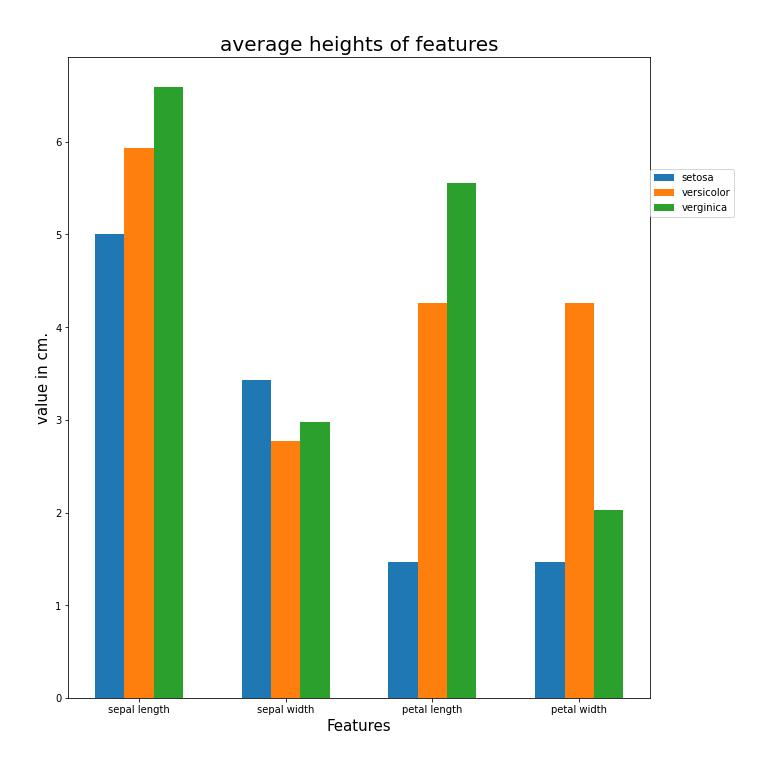
\includegraphics[width=15cm,height=10cm]{mbar.jpeg}

    
\begin{minted}{python}

plt.figure(figsize=(10,10))

plt.subplot(2,2,1)
plt.hist(df["sepal.length"])
plt.xlabel("sepal length(cm)")
plt.ylabel("Frequency")

plt.subplot(2,2,2)
plt.hist(df["sepal.width"],color="orange")
plt.xlabel("sepal width")
plt.ylabel("Frequency")
plt.subplot(2,2,3)
plt.hist(df["petal.length"],color="g")
plt.xlabel("petal length")
plt.ylabel("Frequency")
plt.subplot(2,2,4)
plt.hist(df["petal.width"],color="r")
plt.xlabel("petal lenght")
plt.ylabel("Frequency")
plt.suptitle("Iris Histograms")
plt.savefig("C:\\Users\\shaik\\OneDrive\\Desktop\\itass\\subhists.jpeg",bbox_inches="tight",pad_inches=0.5)
plt.show()
\end{minted}
\newpage
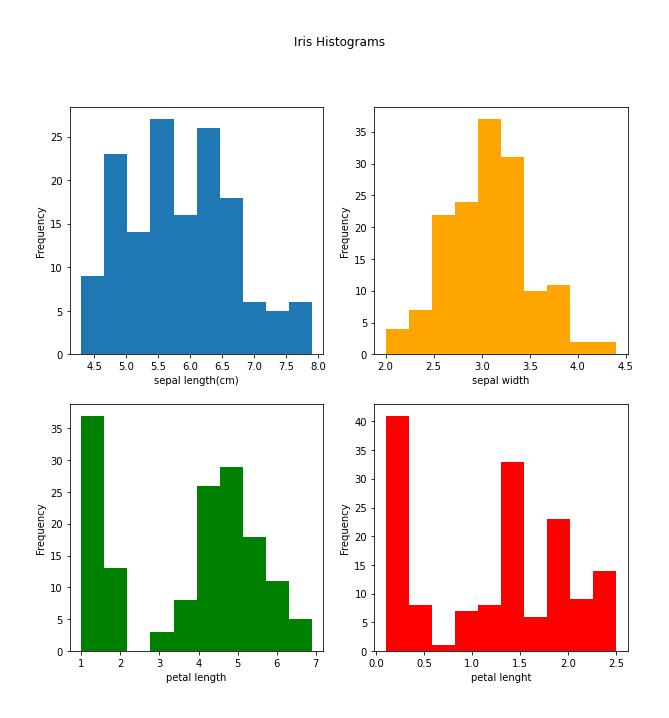
\includegraphics[width=15cm,height=15cm]{subhists.jpeg}
\
\pagestyle{fancy}
\fancyfoot[C]{END}

\end{document}

